        %%******************************************%%
        %%                                          %%
        %%        Modello di tesi di laurea         %%
        %%            di Andrea Giraldin            %%
        %%                                          %%
        %%             2 novembre 2012              %%
        %%                                          %%
        %%******************************************%%


% I seguenti commenti speciali impostano:
% 1. 
% 2. PDFLaTeX come motore di composizione;
% 3. tesi.tex come documento principale;
% 4. il controllo ortografico italiano per l'editor.

% !TEX encoding = UTF-8
% !TEX TS-program = pdflatex
% !TEX root = tesi.tex
% !TEX spellcheck = it-IT

% PDF/A filecontents
\RequirePackage{filecontents}
\begin{filecontents*}{\jobname.xmpdata}
  \Title{Document’s title}
  \Author{Author’s name}
  \Language{it-IT}
  \Subject{The abstract, or short description.}
  \Keywords{keyword1\sep keyword2\sep keyword3}
\end{filecontents*}

\documentclass[10pt,                    % corpo del font principale
               a4paper,                 % carta A4
               twoside,                 % impagina per fronte-retro
               openright,               % inizio capitoli a destra
               english,                 
               italian,                 
               ]{book}    

%**************************************************************
% Importazione package
%************************************************************** 

\PassOptionsToPackage{dvipsnames}{xcolor} % colori PDF/A

\usepackage{colorprofiles}

\usepackage[a-2b,mathxmp]{pdfx}[2018/12/22]
                                        % configurazione PDF/A
                                        % validare in https://www.pdf-online.com/osa/validate.aspx

%\usepackage{amsmath,amssymb,amsthm}    % matematica

\usepackage[T1]{fontenc}                % codifica dei font:
                                        % NOTA BENE! richiede una distribuzione *completa* di LaTeX

\usepackage[utf8]{inputenc}             % codifica di input; anche [latin1] va bene
                                        % NOTA BENE! va accordata con le preferenze dell'editor

\usepackage[english, italian]{babel}    % per scrivere in italiano e in inglese;
                                        % l'ultima lingua (l'italiano) risulta predefinita
                                        
\setcounter{secnumdepth}{3}
     
                                 
\usepackage{float}

\usepackage{bookmark}                   % segnalibri

\usepackage{caption}                    % didascalie

\usepackage{chngpage,calc}              % centra il frontespizio

\usepackage{csquotes}                   % gestisce automaticamente i caratteri (")

\usepackage{emptypage}                  % pagine vuote senza testatina e piede di pagina

\usepackage{epigraph}			% per epigrafi

\usepackage{eurosym}                    % simbolo dell'euro

%\usepackage{indentfirst}               % rientra il primo paragrafo di ogni sezione

\usepackage{graphicx}                   % immagini

\usepackage{hyperref}                   % collegamenti ipertestuali

\usepackage[binding=5mm]{layaureo}      % margini ottimizzati per l'A4; rilegatura di 5 mm

\usepackage{listings}                   % codici

\usepackage{microtype}                  % microtipografia

\usepackage{mparhack,fixltx2e,relsize}  % finezze tipografiche

\usepackage{nameref}                    % visualizza nome dei riferimenti                                      
\usepackage[font=small]{quoting}        % citazioni

\usepackage{subfig}                     % sottofigure, sottotabelle

\usepackage[italian]{varioref}          % riferimenti completi della pagina

\usepackage{booktabs}                   % tabelle                                       
\usepackage{tabularx}                   % tabelle di larghezza prefissata                                    
\usepackage{longtable}                  % tabelle su più pagine                                        
\usepackage{ltxtable}                   % tabelle su più pagine e adattabili in larghezza
\usepackage{colortbl}					% tabelle con righe colorate
\usepackage{enumitem}					% cambiare il margine degli elenchi nelle tabelle

\newcolumntype{C}[1]{>{\centering\let\newline\\\arraybackslash\hspace{0pt}}m{#1}}
\newcolumntype{R}[1]{>{\raggedleft\let\newline\\\arraybackslash\hspace{0pt}}m{#1}}
\newcolumntype{L}[1]{>{\raggedright\let\newline\\\arraybackslash\hspace{0pt}}m{#1}}

\definecolor{bugWhite}{HTML}{f8f3ed}
\definecolor{lighter-bugBlue}{HTML}{d5e8f6}

\usepackage[toc, acronym]{glossaries}   % glossario
                                        % per includerlo nel documento bisogna:
                                        % 1. compilare una prima volta tesi.tex;
                                        % 2. eseguire: makeindex -s tesi.ist -t tesi.glg -o tesi.gls tesi.glo
                                        % 3. eseguire: makeindex -s tesi.ist -t tesi.alg -o tesi.acr tesi.acn
                                        % 4. compilare due volte tesi.tex.

\usepackage[backend=biber,style=verbose-ibid,hyperref,backref]{biblatex}
                                        % eccellente pacchetto per la bibliografia; 
                                        % produce uno stile di citazione autore-anno; 
                                        % lo stile "numeric-comp" produce riferimenti numerici
                                        % per includerlo nel documento bisogna:
                                        % 1. compilare una prima volta tesi.tex;
                                        % 2. eseguire: biber tesi
                                        % 3. compilare ancora tesi.tex.
\usepackage{fancyvrb}
\usepackage{cjkutf8-ko}
%**************************************************************
% file contenente le impostazioni della tesi
%**************************************************************

%**************************************************************
% Frontespizio
%**************************************************************

% Autore
\newcommand{\myName}{Nicla Faccioli}                                    
\newcommand{\myTitle}{Integrazione di Amazon Rekognition e Lex all’interno di una web app basata su AWS Lambda}

% Tipo di tesi                   
\newcommand{\myDegree}{Tesi di laurea triennale}

% Università             
\newcommand{\myUni}{Università degli Studi di Padova}

% Facoltà       
\newcommand{\myFaculty}{Corso di Laurea in Informatica}

% Dipartimento
\newcommand{\myDepartment}{Dipartimento di Matematica "Tullio Levi-Civita"}

% Titolo del relatore
\newcommand{\profTitle}{Prof. }

% Relatore
\newcommand{\myProf}{Lamberto Ballan}

% Luogo
\newcommand{\myLocation}{Padova}

% Anno accademico
\newcommand{\myAA}{2021-2022}

% Data discussione
\newcommand{\myTime}{Luglio 2022}

\newcommand{\azienda}{Zero12 S.r.l. }

%**************************************************************
% Impostazioni di impaginazione
% see: http://wwwcdf.pd.infn.it/AppuntiLinux/a2547.htm
%**************************************************************

\setlength{\parindent}{14pt}   % larghezza rientro della prima riga
\setlength{\parskip}{0pt}   % distanza tra i paragrafi


%**************************************************************
% Impostazioni di biblatex
%**************************************************************
\bibliography{bibliografia} % database di biblatex 

\defbibheading{bibliography} {
	\cleardoublepage
	\phantomsection 
	\addcontentsline{toc}{chapter}{\bibname}
	\chapter*{\bibname\markboth{\bibname}{\bibname}}
}

\setlength\bibitemsep{1.5\itemsep} % spazio tra entry

\DeclareBibliographyCategory{opere}
\DeclareBibliographyCategory{web}

\addtocategory{opere}{womak:lean-thinking}
\addtocategory{web}{site:agile-manifesto}

\defbibheading{opere}{\section*{Riferimenti bibliografici}}
\defbibheading{web}{\section*{Siti Web consultati}}


%**************************************************************
% Impostazioni di caption
%**************************************************************
\captionsetup{
	tableposition=top,
	figureposition=bottom,
	font=small,
	format=hang,
	labelfont=bf
}

%**************************************************************
% Impostazioni di glossaries
%**************************************************************
%**************************************************************
% Glossario
%**************************************************************
%\renewcommand{\glossaryname}{Glossario}

\newglossaryentry{API}
{
	name=API,
	text=Application Program Interface,
	sort=api,
	description={in informatica con il termine \emph{Application Programming Interface API} (ing. interfaccia di programmazione di un'applicazione) si indica ogni insieme di procedure disponibili al programmatore, di solito raggruppate a formare un set di strumenti specifici per l'espletamento di un determinato compito all'interno di un certo programma. La finalità è ottenere un'astrazione, di solito tra l'hardware e il programmatore o tra software a basso e quello ad alto livello semplificando così il lavoro di programmazione}
}



\newglossaryentry{AWS}
{
	name=AWS,
	description={azienda di proprietà Amazon che fornisce servizi di cloud computig, disponibili sull'omonima piattaforma}
}

\newglossaryentry{serverless}
{
	name=serverless,
	description={modello di esecuzione cloud che non richiede la presenza di server fisici che devono essere mantenuti e configurati. I server sono comunuque presetni ma si trovano nel cloud e allocano risorse dinamicamente appena queste vengono richieste. Quando l'applicazione non è in uso, nessuna risorsa viene consumata ed il prezzo risulta quindi essere pari a zero}
}

\newglossaryentry{framework}
{
	name=framework,
	description={architettura logica riutilizzabile sulla quale un software può essere progettato. È definito da un insieme di classi astratte e dalle relazioni tra di esse e può includere programmi, librerie e strumenti di supporto}
}

\newglossaryentry{FaaS}
{
	name=FaaS,
	description={categoria dello sviluppo cloud che fornisce una piattaforma che permetta agli sviluppatori di eseguire e gestire le varie funzionalità della propria applicazione senza necessità di gestire e mantenere infrastrutture fisiche. \emph{FaaS} è una delle modalità con cui si può costruire un'architettura \gls{serverless}}
}

\newglossaryentry{YAML}
{
	name=YAML,
	description={con l’acronimo ricorsivo (\emph{YAML Ain’t a Markup Language}) formato per la serializzazione di dati leggibile da esseri umani. Questo formato può essere utilizzato come file di configurazione, come nel caso del \emph{Serverless Framework}}
}

\newglossaryentry{automatic speech recognition}
{
	name=Automatic Speech Recognition,
	description={prova}
}

\newglossaryentry{natural language understanding}
{
	name=Natural Language Understanding,
	description={prova}
}

\newglossaryentry{skill}
{
	name=skill,
	description={prova}
}

\newglossaryentry{chatbot}
{
	name=chatbot,
	description={prova}
}

\newglossaryentry{NoSQL}
{
	name=NoSQL,
	description={prova}
}

\newglossaryentry{prefisso}
{
	name=prefisso,
	description={prova}
}

\newglossaryentry{deploy}
{
	name=deploy,
	description={prova}
}

\newglossaryentry{CSS}
{
	name=CSS,
	description={prova}
}

\newglossaryentry{HTML}
{
	name=HTML,
	description={prova}
}

\newglossaryentry{controllo di versione}
{
	name=controllo di versione,
	description={prova}
}

\newglossaryentry{repository}
{
	name=repository,
	description={prova}
} % database di termini
\makeglossaries


%**************************************************************
% Impostazioni di graphicx
%**************************************************************
\graphicspath{{immagini/}} % cartella dove sono riposte le immagini


%**************************************************************
% Impostazioni di hyperref
%**************************************************************
\hypersetup{
	%hyperfootnotes=false,
	%pdfpagelabels,
	%draft,	% = elimina tutti i link (utile per stampe in bianco e nero)
	colorlinks=true,
	linktocpage=true,
	pdfstartpage=1,
	pdfstartview=,
	% decommenta la riga seguente per avere link in nero (per esempio per la stampa in bianco e nero)
	%colorlinks=false, linktocpage=false, pdfborder={0 0 0}, pdfstartpage=1, pdfstartview=FitV,
	breaklinks=true,
	pdfpagemode=UseNone,
	pageanchor=true,
	pdfpagemode=UseOutlines,
	plainpages=false,
	bookmarksnumbered,
	bookmarksopen=true,
	bookmarksopenlevel=1,
	hypertexnames=true,
	pdfhighlight=/O,
	%nesting=true,
	%frenchlinks,
	urlcolor=webbrown,
	linkcolor=RoyalBlue,
	citecolor=webgreen,
	%pagecolor=RoyalBlue,
	%urlcolor=Black, linkcolor=Black, citecolor=Black, %pagecolor=Black,
	pdftitle={\myTitle},
	pdfauthor={\textcopyright\ \myName, \myUni, \myFaculty},
	pdfsubject={},
	pdfkeywords={},
	pdfcreator={pdfLaTeX},
	pdfproducer={LaTeX}
}

%**************************************************************
% Impostazioni di itemize
%**************************************************************
\renewcommand{\labelitemi}{$\ast$}

%\renewcommand{\labelitemi}{$\bullet$}
%\renewcommand{\labelitemii}{$\cdot$}
%\renewcommand{\labelitemiii}{$\diamond$}
%\renewcommand{\labelitemiv}{$\ast$}


%**************************************************************
% Impostazioni di listings
%**************************************************************
\lstset{
	language=[LaTeX]Tex,%C++,
	keywordstyle=\color{RoyalBlue}, %\bfseries,
	basicstyle=\small\ttfamily,
	%identifierstyle=\color{NavyBlue},
	commentstyle=\color{Green}\ttfamily,
	stringstyle=\rmfamily,
	numbers=none, %left,%
	numberstyle=\scriptsize, %\tiny
	stepnumber=5,
	numbersep=8pt,
	showstringspaces=false,
	breaklines=true,
	frameround=ftff,
	frame=single
} 


%**************************************************************
% Impostazioni di xcolor
%**************************************************************
\definecolor{webgreen}{rgb}{0,.5,0}
\definecolor{webbrown}{rgb}{.6,0,0}


%**************************************************************
% Altro
%**************************************************************

\newcommand{\omissis}{[\dots\negthinspace]} % produce [...]

% eccezioni all'algoritmo di sillabazione
\hyphenation
{
	ma-cro-istru-zio-ne
	gi-ral-din
}

\newcommand{\sectionname}{sezione}
\addto\captionsitalian{\renewcommand{\figurename}{Figura}
	\renewcommand{\tablename}{Tabella}}

\newcommand{\glsfirstoccur}{\ap{{[g]}}}

\newcommand{\intro}[1]{\emph{\textsf{#1}}}

%**************************************************************
% Environment per ``rischi''
%**************************************************************
\newcounter{riskcounter}                % define a counter
\setcounter{riskcounter}{0}             % set the counter to some initial value

%%%% Parameters
% #1: Title
\newenvironment{risk}[1]{
	\refstepcounter{riskcounter}        % increment counter
	\par \noindent                      % start new paragraph
	\textbf{\arabic{riskcounter}. #1}   % display the title before the 
	% content of the environment is displayed 
}{
	\par\medskip
}

\newcommand{\riskname}{Rischio}

\newcommand{\riskdescription}[1]{\textbf{\\Descrizione:} #1.}

\newcommand{\risksolution}[1]{\textbf{\\Soluzione:} #1.}

%**************************************************************
% Environment per ``use case''
%**************************************************************
\newcounter{usecasecounter}             % define a counter
\setcounter{usecasecounter}{0}          % set the counter to some initial value

%%%% Parameters
% #1: ID
% #2: Nome
\newenvironment{usecase}[2]{
	\renewcommand{\theusecasecounter}{\usecasename #1}  % this is where the display of 
	% the counter is overwritten/modified
	\refstepcounter{usecasecounter}             % increment counter
	\vspace{10pt}
	\par \noindent                              % start new paragraph
	{\large \textbf{\usecasename #1: #2}}       % display the title before the 
	% content of the environment is displayed 
	\medskip
}{
	\medskip
}

\newcommand{\usecasename}{UC}

\newcommand{\usecaseactors}[1]{\textbf{\\Attori Principali:} #1. \vspace{4pt}}
\newcommand{\usecasepre}[1]{\textbf{\\Precondizioni:} #1. \vspace{4pt}}
\newcommand{\usecasedesc}[1]{\textbf{\\Descrizione:} #1. \vspace{4pt}}
\newcommand{\usecasepost}[1]{\textbf{\\Postcondizioni:} #1. \vspace{4pt}}
\newcommand{\usecasealt}[1]{\textbf{\\Scenario Alternativo:} #1. \vspace{4pt}}

%**************************************************************
% Environment per ``namespace description''
%**************************************************************

\newenvironment{namespacedesc}{
	\vspace{10pt}
	\par \noindent                              % start new paragraph
	\begin{description} 
	}{
	\end{description}
	\medskip
}

\newcommand{\classdesc}[2]{\item[\textbf{#1:}] #2}
                     % file con le impostazioni personali

\begin{document}
%**************************************************************
% Materiale iniziale
%**************************************************************
\frontmatter
% !TEX encoding = UTF-8
% !TEX TS-program = pdflatex
% !TEX root = ../tesi.tex

%**************************************************************
% Frontespizio 
%**************************************************************
\begin{titlepage}
	
	\begin{center}
		
		\begin{LARGE}
			\textbf{\myUni}\\
		\end{LARGE}
		
		\vspace{10pt}
		
		\begin{Large}
			\textsc{\myDepartment}\\
		\end{Large}
		
		\vspace{10pt}
		
		\begin{large}
			\textsc{\myFaculty}\\
		\end{large}
		
		\vspace{30pt}
		\begin{figure}[htbp]
			\begin{center}
				
\includegraphics[height=5.5cm]{logo-unipd}
			\end{center}
		\end{figure}
		\vspace{30pt} 
		
		\begin{LARGE}
			\begin{center}
				\textbf{\myTitle}\\
			\end{center}
		\end{LARGE}
		
		\vspace{10pt} 
		
		\begin{large}
			\textsl{\myDegree}\\
		\end{large}
		
		\vspace{40pt} 
		
		\begin{large}
			\begin{flushleft}
				\textit{Relatore}\\ 
				\vspace{5pt} 
				\profTitle \myProf
			\end{flushleft}
			
			\vspace{0pt} 
			
			\begin{flushright}
				\textit{Laureanda}\\ 
				\vspace{5pt} 
				\myName
			\end{flushright}
		\end{large}
		
		\vspace{35pt}
		
		\line(1, 0){338} \\
		\begin{normalsize}
			\textsc{Anno Accademico \myAA}
		\end{normalsize}
		
	\end{center}
\end{titlepage} 
% !TEX encoding = UTF-8
% !TEX TS-program = pdflatex
% !TEX root = ../tesi.tex

%**************************************************************
% Colophon
%**************************************************************
\clearpage
\phantomsection
\thispagestyle{empty}

\hfill

\vfill

\noindent\myName: \textit{\myTitle,}
\myDegree,
\textcopyright\ \myTime.
% !TEX encoding = UTF-8
% !TEX TS-program = pdflatex
% !TEX root = ../tesi.tex

%**************************************************************
% Sommario
%**************************************************************
\cleardoublepage
\phantomsection
\pdfbookmark{Sommario}{Sommario}
\begingroup
\let\clearpage\relax
\let\cleardoublepage\relax
\let\cleardoublepage\relax

\chapter*{Sommario}

Il presente documento descrive l’attività di stage svolta presso l’azienda Zero12 s.r.l. Lo stage è stato svolto alla conclusione del percorso di studi della laurea triennale in Informatica ed ha avuto la durata di circa trecento ore. L’obiettivo dello stage è stato l’integrazione dei servizi AWS di image recognition (Amazon Rekognition), automatic speech recognition e natural language understanding (Amazon Lex) all’interno di un’applicazione web serverless basata su AWS Lambda con lo scopo di facilitare l’inserimento dei dati. 

%\vfill
%
%\selectlanguage{english}
%\pdfbookmark{Abstract}{Abstract}
%\chapter*{Abstract}
%
%\selectlanguage{italian}

\endgroup			

\vfill


% !TEX encoding = UTF-8
% !TEX TS-program = pdflatex
% !TEX root = ../tesi.tex

%**************************************************************
% Ringraziamenti
%**************************************************************
\cleardoublepage
\phantomsection
\pdfbookmark{Ringraziamenti}{ringraziamenti}

\begin{flushright}{
	\slshape    
	``Let us light up the night, we shine in our own ways. \\
		Shine, dream, smile''} \\ 
	\medskip
    --- 방탄소년단
\end{flushright}


\bigskip

\begingroup
\let\clearpage\relax
\let\cleardoublepage\relax
\let\cleardoublepage\relax

\chapter*{Ringraziamenti}

\noindent \textit{Innanzitutto, vorrei esprimere la mia gratitudine al \profTitle \myProf, relatore della mia tesi, per l'aiuto e il sostegno fornitomi durante la stesura del lavoro.}\\

\noindent \textit{Desidero ringraziare tutta la mia enorme famiglia ingrandita per avermi sempre sostenuta in ogni mia scelta e per avermi dato il coraggio necessario ad andare avanti. Grazie per tutti gli insegnamenti che mi avete trasmesso e che mi hanno permesso di raggiungere questo traguardo. \\
 	Un grazie speciale va alla mia mamma che, nonostante le difficoltà, gli imprevisti e il percorso dissestato che ho affrontato, mi ha sempre incoraggiata, ha creduto in me e ha saputo sdrammatizzare nei momenti che sembravano insuperabili. Grazie mamma per essere non solo una madre ma anche un'amica, sempre al mio fianco e pronta a farsi in quattro per aiutarmi a realizzare ogni mio sogno. \\
 	Grazie anche a papà per l'interesse che mostri ogni volta che ti racconto gli argomenti che studio, i progetti che realizzo o le cose che mi interessano. Grazie per esserci sempre quando ho bisogno di consigli o semplicemente di chiacchierare e condividere i miei pensieri. \\
	Grazie a mio fratello Simone che con le sue chiamate serali interminabili non mi ha mai fatto sentire poi così lontana da casa. Grazie per avermi continuato a rendere partecipe di ogni parte della tua vita nonostante la distanza che ci separa e per essere così partecipe nella mia.}\\
 
\noindent \textit{Vorrei ringraziare anche tutti i miei amici e le mie amiche per le mille avventure vissute in questi anni.} \\
\noindent \textit{In particolar modo Anna che mi ha sopportato come coinquilina e compagna di stanza. Grazie per essere non solo la miglior coinquilina che si possa desiderare, ma anche una delle mie migliori amiche e una grande confidente. Grazie per essermi sempre stata vicina, per avermi ascoltato quando ne avevo bisogno e per aver condiviso con me tante risate, tanta ansia e anche qualche lacrima.}\\                                                                                                
\noindent \textit{Un grazie anche a Giorgia che ha condiviso con me ogni giorno di vita universitaria sin dal principio. Grazie per tutte le avventure nate da idee pazze che abbiamo avuto insieme e per essere sempre pronta a partire per qualsiasi luogo che ci venga in mente, da Banzai in centro a Padova fino al Giappone.}\\
\bigskip

\noindent\textit{\myLocation, \myTime}
\hfill \myName

\endgroup

% !TEX encoding = UTF-8
% !TEX TS-program = pdflatex
% !TEX root = ../tesi.tex

%**************************************************************
% Indici
%**************************************************************
\cleardoublepage
\pdfbookmark{\contentsname}{tableofcontents}
\setcounter{tocdepth}{2}
\tableofcontents
%\markboth{\contentsname}{\contentsname} 
\clearpage

\begingroup 
    \let\clearpage\relax
    \let\cleardoublepage\relax
    \let\cleardoublepage\relax
    %*******************************************************
    % Elenco delle figure
    %*******************************************************    
    \phantomsection
    \pdfbookmark{\listfigurename}{lof}
    \listoffigures

    \vspace*{8ex}

    %*******************************************************
    % Elenco delle tabelle
    %*******************************************************
    \phantomsection
    \pdfbookmark{\listtablename}{lot}
    \listoftables
        
    \vspace*{8ex}
\endgroup

\cleardoublepage

\cleardoublepage

%**************************************************************
% Materiale principale
%**************************************************************
\mainmatter
% !TEX encoding = UTF-8
% !TEX TS-program = pdflatex
% !TEX root = ../tesi.tex

%**************************************************************
\chapter{Introduzione}
\label{cap:introduzione}
%**************************************************************

\section{L'azienda}

\azienda è un'azienda informatica nata nel 2012 specializzata nello sviluppo di soluzioni cloud native, sempre in prima linea nel seguire l'evoluzione di questo paradigma tecnologico. \\
L'azienda è partner \gls{AWS} e si occupa di progettazione e sviluppo software Web e Mobile per clienti provenienti da ambiti molto diversificati. \\
L'obiettivo di \azienda è aiutare i propri clienti a definire percorsi di innovazione includendo le tecnologie più avanzate tra cui per esempio
il cloud ed il machine learning per l'analisi di linguaggio naturale, immagini, video e per fare previsioni. 

	\begin{figure}[H]
		\centering
		
\includegraphics[width=5cm]{immagini/logo-zero12.png} \\
		\caption{\label{fig:logo_zero12} Logo di Zero12 s.r.l.}
	\end{figure}

%**************************************************************
\section{L'offerta di stage}
	Attualmente in azienda è presente una piattaforma denominata MariBa con lo scopo di registrare i risultati di gioco del personale a Mario Kart e calcetto balilla. L'inserimento di tali dati però è completamente manuale: ogni partita va
	inizializzata con l'inserimento dei nickname di tutti i giocatori e, una volta conclusa, i risultati devono
	essere inseriti manualmente all'interno della piattaforma. L'idea dello stage è di semplificare l'inserimento di questi
	dati attraverso l'utilizzo di tecnologie \gls{AWS} per il riconoscimento automatico dei giocatori e per la registrazione dei risultati comunicandoli vocalmente alla piattaforma. \\
	Il progetto è stato proposto dall'azienda in occasione dell'evento Stage-it 2022 (logo in \autoref{fig:logo_stageit}) finalizzato all'incontro tra aziende e studenti.
	
	\begin{figure}[H]
		\centering
		
\includegraphics[width=7cm]{immagini/stageit.png} \\
		\caption{\label{fig:logo_stageit} Logo dell'evento Stage-it 2022}
	\end{figure}

%**************************************************************
\section{Struttura del documento}

	\begin{description}
	    \item[{\hyperref[cap:descrizione-stage]{Il secondo capitolo}}] descrive il progetto di stage e la pianificazione delle attività;
	    
		\item[{\hyperref[cap:tecnologie]{Il terzo capitolo}}] definisce le tecnologie utilizzate durante lo stage;
		
		\item[{\hyperref[cap:applicazione]{Il quarto capitolo}}] approfondisce lo sviluppo del sistema di image recognition;
	    
	    \item[{\hyperref[cap:rekognition]{Il quinto capitolo}}] approfondisce lo sviluppo del sistema di image recognition;
	    
	    \item[{\hyperref[cap:lex]{Il sesto capitolo}}] approfondisce lo sviluppo del sistema di voice service;
	   
	    \item[{\hyperref[cap:conclusioni]{Nel settimo capitolo}}] sono descritte le conclusioni dell'esperienza di stage e gli obiettivi raggiunti.
	\end{description}




             % Introduzione
% !TEX encoding = UTF-8
% !TEX TS-program = pdflatex
% !TEX root = ../tesi.tex

%**************************************************************
\chapter{Descrizione dello stage}
\label{cap:descrizione-stage}
%**************************************************************

%**************************************************************
\section{Introduzione al progetto}
In \azienda è stata creata una piattaforma denominata MariBa con lo scopo di registrare i risultati di gioco del personale a Mario Kart e calcetto balilla. Tale piattaforma è dotata di un sistema di intelligenza artificiale che, in base ai giocatori (o alle coppie nel caso del calcetto), è in grado di predire il risultato del match di gioco. Il limite della
piattaforma attuale è che tutti i dati, dall'inizializzazione di una partita ai risultati finali, devono essere inseriti
manualmente. \\

Al fine di rendere più immediato l'inserimento dei dati si vuole evolvere la piattaforma includendo le seguenti funzionalità:
\begin{itemize}
	\item Sistema di \gls{image recognition} pe riconoscere i giocatori e ruoli durante la fase di inizializzazione della partita
	e formazione delle squadre;
	\item Servizio vocale per l'inserimento dei risultati dei match giocati.
\end{itemize}


%**************************************************************
\section{Obiettivi formativi}
	Gli obiettivi formativi dell'attività di stage sono i seguenti:
	\begin{itemize}
		\item Apprendere come sviluppare un applicativo web con controlli vocali;
		\item Apprendere come svolgere attività di integrazione con servizi di Machine Learning in ambito \gls{image recognition}, \gls{automatic speech recognition} (ASR) e \gls{natural language understanding} (NLU);
	\end{itemize}
%**************************************************************

\section{Requisiti}
Nel primo giorno di stage si è svolto un incontro con il tutor aziendale per definire in modo dettagliato i requisiti. Nel corso dello stage il livello di obbligatorietà di tali requisiti è variato in risposta alle esigenze dell'azienda. \\
 Di seguito viene riportata la versione finale dell'analisi effettuata.

	\subsection{Requisiti obbligatori}
		Di seguito vengono elencati i requisiti obbligatori:
		\begin{itemize}
			\item Sviluppo di un micro-servizio per le attività di \emph{face detection} e \emph{recognition};
			\item Sviluppo di un micro-servizio per le attività di controllo vocale via web
		\end{itemize}
	\subsection{Requisiti desiderabili}
		Di seguito vengono elencati i requisiti desiderabili:
		\begin{itemize}
			\item Integrazione di un nuovo gioco all'interno della piattaforma;
			\item Implementazione di una versione semplificata per l'inserimento dei dati di Mario Kart per l'utilizzo
			della piattaforma in occasione del Summit \gls{AWS} di Milano.
		\end{itemize}
	\subsection{Requisiti facoltativi}
		Di seguito vengono elencati i requisiti facoltativi:
		\begin{itemize}
			\item Sviluppo di una \gls{skill} Alexa con le stesse funzionalità del \gls{chatbot} vocale richiesto come requisito obbligatorio e integrato sulla piattaforma web.
		\end{itemize}

%**************************************************************
\section{Pianificazione}
La durata complessiva dello stage è stata di 8 settimane di lavoro a tempo pieno per un totale di circa 320 ore. \\

\noindent Secondo il piano di lavoro iniziale definito con l'azienda, le attività sono distribuite come segue:

\begin{center}
	
	\renewcommand{\arraystretch}{1.5}
	
		\centering
		\begin{longtable}{| C{2.5cm} | C{2cm} | L{7.2cm} |}
			
			\hline
			
			\rowcolor{lighter-bugBlue}
			\textbf{Durata in ore} & \textbf{Settimana} & \textbf{Descrizione} \\
			
			\hline
			
			40 & 1 &
			\begin{itemize}[leftmargin=*]
				\item Studio delle tecnologie necessarie.
			\end{itemize} \\
			
			\hline
			
			80 & 2, 3 &
			\begin{itemize}[leftmargin=*]
				\item Progettazione e sviluppo di un micro-servizio per attività di \emph{face detection} per 
				la creazione di squadre di gioco;
				\item Integrazione con la piattaforma esistente. 
			\end{itemize}  \\
			
			\hline
		
			
			80 & 4, 5 &
			\begin{itemize}[leftmargin=*]
				\item Progettazione e sviluppo di un micro-servizio per il controllo vocale;
				\item Integrazione con la piattaforma esistente. 
			\end{itemize}  \\
			 
			\hline
			
			80 & 6, 7 &
			\begin{itemize}[leftmargin=*]
				\item Sviluppo della skill Alexa per il controllo vocale e l'aggiornamento dei risultati;
				\item Integrazione con la piattaforma esistente. 
			\end{itemize}  \\
			
			\hline
			
			40 & 8 &
			\begin{itemize}[leftmargin=*]
				\item Testing e stesura della documentazione di progetto delle attività di sviluppo condotte nelle settimane precedenti.
			\end{itemize} \\
			
			\hline
			
			\rowcolor{lighter-bugBlue}
			\multicolumn{2}{ | c | }{\textbf{Totale ore: }} & 	\multicolumn{1}{  c | }{\textbf{320}}\\
			
			\hline
		
			
			\caption{Pianificazione delle attività}
		\end{longtable}
		
	
\end{center}
Durante il periodo di stage in azienda il piano di lavoro ha subito modifiche e di conseguenza la versione finale della pianificazione riportata nel \autoref{cap:conclusioni} diverge da quella qui presentata. Tali modifiche sono state effettuate in risposta alle esigenze e richieste dell'azienda. 
Durante tutta la durata del tirocinio sono stati effettuati stand-up giornalieri con il tutor aziendale in affiancamento per 
monitorare lo stato di avanzamento ed evidenziare eventuali problemi sorti.
             % Descrizione stage
% !TEX encoding = UTF-8
% !TEX TS-program = pdflatex
% !TEX root = ../tesi.tex

%**************************************************************
\chapter{Tecnologie e strumenti}
\label{cap:tecnologie}
%**************************************************************

In questo capitolo vengono presentate le tecnologie utilizzate durante lo stage.\\

%**************************************************************
\section{Tecnologie per il back-end}
	\subsection{Serverless Framework}
	\emph{Serverless Framework} è un \gls{framework} web che permette di costruire applicazioni \gls{serverless} basate sul concetto \gls{FaaS}. Esso permette di definire funzioni Lambda e infrastrutture \gls{AWS} utilizzando sintassi \gls{YAML}.
	
	\begin{figure}[H]
		\centering
		
\includegraphics[width=5cm]{immagini/serverless.png} \\
		\caption{\label{fig:logo_serverless} Logo Serverless Framework}
	\end{figure}
	
	\subsection{Node.js}
	\emph{Node.js} è un ambiente runtime open source per l'esecuzione di codice \emph{JavaScript} all'esterno di browser web. Esso consente infatti di utilizzare \emph{JavaScript} come linguaggio di programmazione lato server. All'interno del progetto
	viene utilizzata la versione 12.x per compatibilità con il codice già presente.
	
	\begin{figure}[H]
		\centering
		
\includegraphics[width=3.3cm]{immagini/nodejs.png} \\
		\caption{\label{fig:logo_node} Logo Node.js}
	\end{figure}
	
	\subsection{AWS Lambda}
	\emph{AWS Lambda} è un servizio di calcolo serverless che permette l'esecuzione di codice per qualsiasi tipo di applicazione o servizio back-end senza bisogno di gestire un'infrastruttura server. \emph{Lambda} gestisce le risorse di elaborazione scalando automaticamente in risposta alla potenza di calcolo richiesta. Il linguaggio utilizzato per lo
	sviluppo di funzioni \emph{Lambda} è \emph{Node.js v12.x}.
	
	\begin{figure}[H]
		\centering
		
\includegraphics[width=2.3cm]{immagini/aws-lambda.png} \\
		\caption{\label{fig:logo_lambda} Logo AWS Lambda}
	\end{figure}
	
	\subsection{Amazon API Gateway}
	\emph{API Gateway} è un servizio Amazon che consente di creare \emph{API RESTful} per permettere una comunicazione bidirezionale in tempo reale tra applicazioni e servizi di back-end. Le \gls{API} definite nell'applicazione sviluppata sono state
	integrate alle rispettive funzioni \emph{Lambda}.
	
	\begin{figure}[H]
		\centering
		
\includegraphics[width=2.2cm]{immagini/api-gateway.png} \\
		\caption{\label{fig:logo_apigateway} Logo Amazon API Gateway}
	\end{figure}
	
	\subsection{Amazon DynamoDB}
	\emph{DynamoDB} è un database \gls{NoSQL}, \gls{serverless}, completamente gestito che supporta l'inserimento di dati di tipo chiave-valore. Facendo parte della famiglia di servizi messi a disposizione da Amazon, \emph{DynamoDB} si integra senza
	difficoltà con tutti i servizi \gls{AWS} e Amazon.
	
	\begin{figure}[H]
		\centering
		
\includegraphics[width=2.5cm]{immagini/DynamoDB.png} \\
		\caption{\label{fig:logo_dynamoDB} Logo Amazon DynamoDB}
	\end{figure}
	
	\subsection{Amazon S3}
	\emph{Amazon Simple Storage Service} (S3) è un servizio di archiviazione di oggetti, scalabile, sicuro e con ottime prestazioni. Al suo interno i dati sono organizzati in \emph{bucket}. All'interno di ogni \emph{bucket} è possibile definire dei prefissi per poter organizzare al meglio gli oggetti caricati. \\
	All'intero del progetto questo servizio è stato utilizzato per effettuare l’hosting della web app e per il trasferimento indiretto di immagini e audio tra front-end e back-end.
	
	\begin{figure}[H]
		\centering
		
\includegraphics[width=2.4cm]{immagini/amazon-s3.png} \\
		\caption{\label{fig:logo_s3} Logo Amazon S3}
	\end{figure}

	
	\subsection{Amazon Rekognition}
	\emph{Amazon Rekognition} è un software \emph{cloud-based} che mette a disposizione capacità di visione artificiale pre-addestrate e personalizzabili per estrarre informazioni dettagliate da immagini e video. Alcuni esempi di utilizzo sono la moderazione di contenuti e \emph{sentiment analysis}.\\ 
	All'interno del progetto è stato utilizzato per implementare la ricerca di volti all'interno di fotografie e per il loro riconoscimento in fase di inizializzazione di una partita e inserimento dei giocatori.
	
	\begin{figure}[H]
		\centering
		
\includegraphics[width=2.5cm]{immagini/rekognition.png} \\
		\caption{\label{fig:logo_rekognition} Logo Amazon Rekognition}
	\end{figure}
	
	\subsection{Amazon Lex}
	\emph{Amazon Lex} è un servizio di intelligenza artificiale completamente gestito che mette a disposizione modelli avanzati di linguaggio naturale. Questo permette di sviluppare interfacce di comunicazione all'interno di applicazioni software. Nel progetto è stato utilizzato per implementare un \gls{chatbot} vocale in modo che 
	l'utente potesse interagire con MariBa e registrare i risultati delle partite giocate.
	
	\begin{figure}[H]
		\centering
		
\includegraphics[width=2.4cm]{immagini/lex.png} \\
		\caption{\label{fig:logo_lex} Logo Amazon Lex}
	\end{figure}

\section{Tecnologie per il front-end}
	\subsection{TypeScript}
	\emph{TypeScript} è un linguaggio di programmazione sviluppato e manutenuto da Microsoft. \\
	Esso è un estensione del linguaggio di programmazione \emph{JavaScript}: utilizza la stessa sintassi ma con l'aggiunta del supporto alla tipizzazione e alle interfacce. 
	
	\begin{figure}[H]
		\centering
		
\includegraphics[width=2cm]{immagini/typescript.png} \\
		\caption{\label{fig:logo_typescript} Logo TypeScript}
	\end{figure}

	\subsection{Angular}
	\emph{Angular} è un \gls{framework} open-source sviluppato da Google. Esso permette lo sviluppo di applicazioni web organizzate in componenti attraverso l'utilizzo di \emph{TypeScript}, \gls{HTML} e \gls{CSS}.
	
	\begin{figure}[H]
		\centering
		
\includegraphics[width=2.5cm]{immagini/angular.png} \\
		\caption{\label{fig:logo_angular} Logo Angular}
	\end{figure}

	\subsection{Nebular}
	\emph{Nebular} è una libreria di \emph{Angular} gratuita e open-source per la creazione di interfacce utente.
	
	\begin{figure}[H]
		\centering
		
\includegraphics[width=1.8cm]{immagini/nebular.png} \\
		\caption{\label{fig:logo_nebular} Logo Nebular}
	\end{figure}


\section{Strumenti di supporto a progettazione e codifica}
	\subsection{Git}
	\emph{Git} è un sistema di \gls{controllo di versione} distribuito. \emph{Git} permette di tenere traccia di tutte le modifiche avvenute all'interno di un progetto o di un singolo file e associa a ciascuna di esse il relativo autore. Permette inoltre di tornare ad una versione precedente del software eliminando le modifiche effettuate successivamente allo stato desiderato. Tutto ciò rende più semplice la collaborazione tra sviluppatori nella stesura del codice durante la fase di sviluppo software.
	
	\begin{figure}[H]
		\centering
		
\includegraphics[width=2cm]{immagini/git.png} \\
		\caption{\label{fig:logo_git} Logo Git}
	\end{figure}

	\subsection{AWS CodeCommit}
	\emph{CodeCommit} è un servizio gestito, altamente scalabile e sicuro che consente l'hosting di \emph{repository} \emph{Git} privati. Esso custodisce i \emph{repository} nel cloud \gls{AWS} e supporta tutti i comandi \emph{Git}. Si è scelto di utilizzare \emph{CodeCommit} rispetto ad altri servizi equivalenti per compatibilità con la scelta aziendale e con il progetto esistente.
	
	\begin{figure}[H]
		\centering
		
\includegraphics[width=2cm]{immagini/codecommit.png} \\
		\caption{\label{fig:logo_codecommit} Logo AWS CodeCommit}
	\end{figure}

	\subsection{VisualStudio Code}
\emph{Visual Studio Code} (VS Code) è un editor per il codice sorgente sviluppato da Microsoft. Esso possiede un controllo per \emph{Git} integrato e mette a disposizione numerose estensioni per facilitare la stesura del codice. Un esempio è \emph{Prettier}, estensione che automatizza la formattazione del codice in modo da mantenerlo ordinato e con uno stile consistente.
	
	\begin{figure}[H]
		\centering
		
\includegraphics[width=2cm]{immagini/visual-studio-code.png} \\
		\caption{\label{fig:logo_vscode} Logo Visual Studio Code}
	\end{figure}

	\subsection{Balsamiq Wireframes}
	\emph{Balsamiq Wireframes} è uno strumento grafico per la creazione di schizzi per interfacce utente e schermate (\emph{wireframes}) di siti web e applicazioni. Durante lo stage è stata utilizzata la versione cloud. I \emph{wireframes} creati sono stati revisionati dal tutor aziendale, il quale ha potuto inserire commenti sulle modifiche da apportare. 
	
		\begin{figure}[H]
		\centering
		
\includegraphics[width=2cm]{immagini/balsamiq.png} \\
		\caption{\label{fig:logo_balsamiq} Logo Balsamiq}
	\end{figure}
	










             % tecnologie e strumenti
% !TEX encoding = UTF-8
% !TEX TS-program = pdflatex
% !TEX root = ../tesi.tex

%**************************************************************
\chapter{Descrizione dell'applicativo}
\label{cap:applicazione}
%**************************************************************

In questo capitolo viene descritto l'applicativo le cui funzionalità sono state estese durante lo stage.\\

\section{Architettura serverless}
L'architettura della web app è basata sul \emph{Serverless Framework} che, come suggerisce il nome, è un \gls{framework} che permette di costruire architetture \gls{serverless}. Esso consente inoltre di definire l'architettura \gls{AWS} (tabelle \emph{DynamoDB}, funzioni \emph{Lambda} e bucket \emph{S3}) attraverso un file in formato \gls{YAML}. \\
 Nei paragrafi seguenti vengono mostrati alcuni esempi della sintassi per la definizione delle infrastrutture necessarie ai nuovi servizi implementati ed il procedimento da seguire per effettuare il \gls{deploy} della struttura \gls{serverless}.
	\subsection{Definizione delle resources}
	Attraverso la direttiva \emph{ Resources} è possibile definire le risorse a cui le funzioni \emph{Lambda} possono accedere, ovvero tabelle \emph{DynamoDB} e \emph{bucket S3} .
	
		\subsubsection{Tabelle DynamoDB}
		\begin{figure}[H]
			\centering
			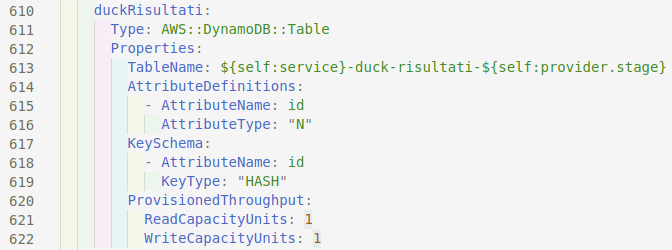
\includegraphics[width=11cm]{immagini/tabellaDB.png} \\
			\caption{\label{fig:tabellaDB} Esempio del codice per la creazione di una tabella DynamoDB}
		\end{figure}
		
		Nel codice sopra riportato:
		\begin{itemize}
			\item \textbf{Type} definisce il tipo di risorsa da creare;
			\item \textbf{TableName} indica il nome della tabella riportato nei servizi \gls{AWS};
			\item \textbf{AttributeDefinitions} descrive gli attributi che compongono la chiave primaria;
			\item \textbf{KeySchema} definisce la struttura della chiave primaria. Nell'esempio la chiave è composta da un solo attributo ma \emph{DynamoDB} permette di definire anche chiavi più complesse;
			\item \textbf{ProvisionedThroughput} specifica il numero di letture e scritture permesse della risorsa.
		\end{itemize}

		\subsubsection{Bucket S3} \label{subsec:bucketS3}
			
		\begin{figure}[H]
			\centering
			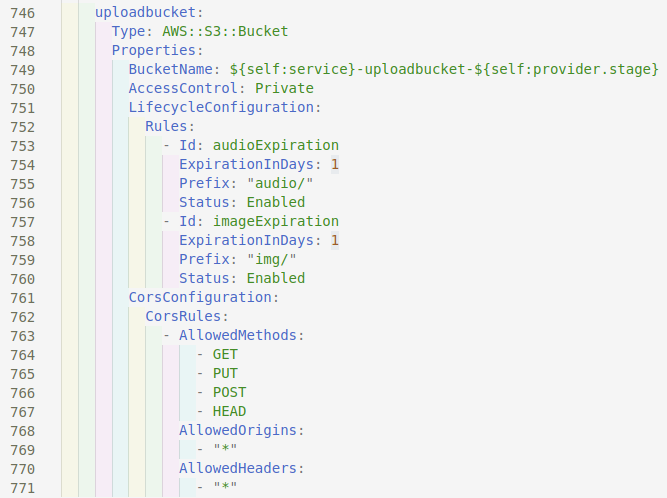
\includegraphics[width=11cm]{immagini/bucketS3.png} \\
			\caption{\label{fig:bucketS3} Esempio del codice per la creazione di un bucket S3}
		\end{figure}
	
		Nel codice sopra riportato:
		\begin{itemize}
			\item \textbf{Type} definisce il tipo di risorsa da creare;
			\item \textbf{BucketName} indica il nome del \emph{bucket} riportato nei servizi \gls{AWS};
			\item \textbf{AccessControl} specifica i permessi di accesso al \emph{bucket};
			\item \textbf{LifeCycleConfiguration} permette di definire delle regole per il ciclo di vita degli oggetti all'interno del bucket. Nel caso riportato sono state definite due regole per due diversi prefissi all'interno del \emph{bucket} (\emph{audioExpiration} e \emph{imageExpiration}) entrambe con durata di un giorno;
			\item \textbf{CorsConfiguration} descrive le configurazione per le \gls{CORS} per gli oggetti del \emph{bucket}.
		\end{itemize}
	
	\subsection{Definizione delle funzioni Lambda}
	Per definire le funzioni \emph{Lambda} viene utilizzata la direttiva \emph{functions}. 
	
	\begin{figure}[H]
		\centering
		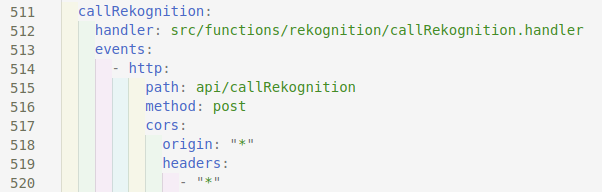
\includegraphics[width=11cm]{immagini/lambda.png} \\
		\caption{\label{fig:lambda} Esempio del codice per la creazione di una funzione Lambda}
	\end{figure}

	Nel codice sopra riportato:
	\begin{itemize}
		\item \textbf{handler} è il riferimento al file contenente il codice della funzione; 
		\item \textbf{events} indica gli eventi che causano l'esecuzione della funzione \emph{Lambda}. In particolare permette di specificare:
		\begin{itemize}
			\item \textbf{http}: definisce gli \emph{API Gateway} HTTP endpoint che quando chiamati provocano l'esecuzione della funzione;
			\item \textbf{path}: definisce il path dell'endpoint e identifica la risorsa;
			\item \textbf{method}: indica il tipo di accesso HTTP permesso;
			\item \textbf{cors}: abilita le \gls{CORS}.
		\end{itemize}
		 
	\end{itemize}
	
	\subsection{Deploy del back-end}
	Per effettuare il \gls{deploy} delle modifiche alle funzioni e alle risorse definite nel file \emph{serverless.yml} è sufficiente eseguire il comando
	\begin{center}
		\texttt{serverless deploy}.
	\end{center} 
	In alternativa, per fare il \gls{deploy} di singole funzioni è possibile eseguire il comando 
	\begin{center}
		\texttt{serverless deploy function -f <nome della funzione>}.
	\end{center}

\section{Web app}
La web app è realizzata utilizzando \emph{Angular 12.x} in collaborazione con \emph{Nebular}, libreria per la realizzazione di interfacce utente. \\
Nei paragrafi successivi vengono descritte le funzionalità disponibili all'interno dell'applicativo, in parte già presenti prima dell'inizio del tirocinio. Viene inoltre mostrato come effettuare il \gls{deploy} delle modifiche effettuate al front-end.
	\subsection{Funzionalità disponibili}
		\paragraph{Salvataggio dei risultati} ~\smallskip 
		
		\noindent All'interno dell'applicativo era già presente la possibilità di inserire i risultati delle partite giocate a due giochi differenti: Mario Kart e Calcetto. Durante lo stage, l'applicativo è stato esteso includendo la possibilità di caricare i risultati anche per un terzo gioco: Duck Game.
		Tutti i risultati inseriti vengono memorizzati all'interno di tabelle \emph{DynamoDB} dedicate e successivamente utilizzati per
		aggiornare il punteggio \gls{Elo} dei giocatori che hanno partecipato.
		
		\begin{figure}[H]
			\centering
			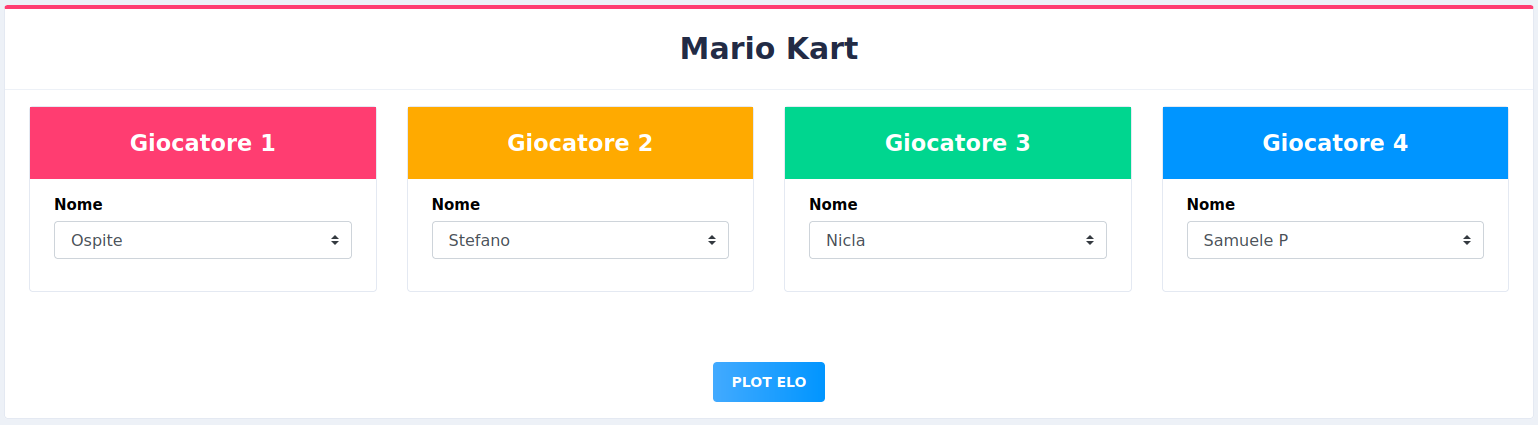
\includegraphics[width=\textwidth]{immagini/insPartita.png} \\
			\caption{\label{fig:inserimento} Form per l'inserimento di una nuova partita}
		\end{figure}
		
		\paragraph{Predizione dei risultati di nuove partite} ~\smallskip 
		
		\noindent Nell'applicativo viene utilizzato un algoritmo di \emph{Machine Learning} che, sfruttando i punteggi \gls{Elo} dei giocatori partecipanti, è in grado di predire i risultati della partita.
		Ogni volta che vengono inserite nuove partite, l'algoritmo migliora le proprie predizioni diventando sempre più preciso. 
		
		\begin{figure}[H]
			\centering
			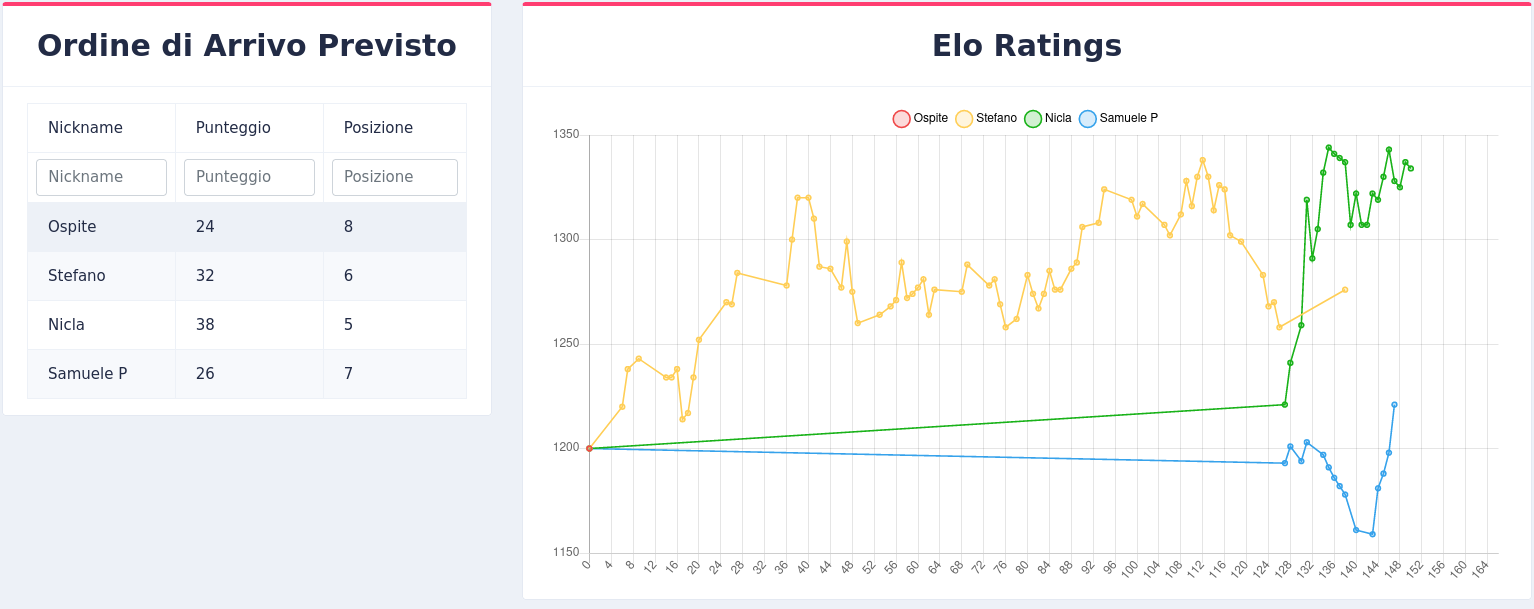
\includegraphics[width=\textwidth]{immagini/predizione.png} \\
			\caption{\label{fig:predizione} Visualizzazione della predizione di una nuova partita}
		\end{figure}
		
		\paragraph{Visualizzazione delle statistiche} ~\smallskip 
		
		\noindent Per ciascun gioco supportato all'interno della web app è presente la pagina \emph{\gls{Elo} rating}
		che permette di visualizzare i punteggi \gls{Elo} di tutti i giocatori. Inoltre, all'interno della stessa 
		pagina, viene mostrato un grafico con lo storico di tutti i punteggi per i dieci giocatori più frequenti nello specifico gioco scelto.
		
		\begin{figure}[H]
			\centering
			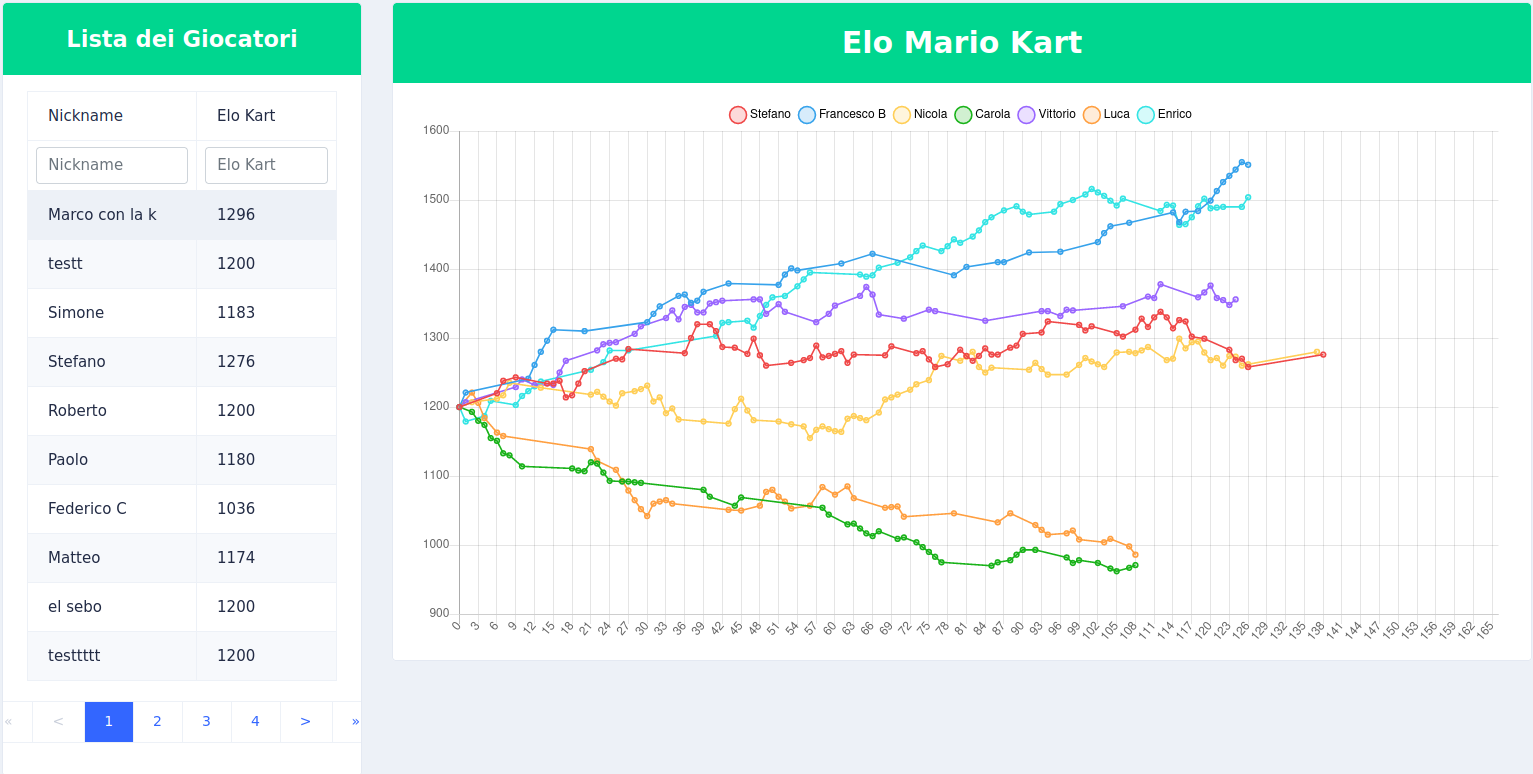
\includegraphics[width=\textwidth]{immagini/elo.png} \\
			\caption{\label{fig:elo} Pagina per la visualizzazione dei punteggi Elo}
		\end{figure}
		
		
	\subsection{Deploy del front-end}
	Per eseguire il \gls{deploy} delle modifiche al front-end è necessario seguire i seguenti passi:
	\begin{enumerate}
		\item Nella cartella del progetto, generare la cartella \emph{dist} eseguendo il comando
		\begin{center}
			\texttt{ng build}
		\end{center}
		\item Utilizzare la console \gls{AWS} per visualizzare il contenuto del \emph{bucket} in cui è stato eseguito l'hosting del sito;
		\item Sostituire il contenuto del \emph{bucket} con i file presenti nella cartella \emph{dist} generata;
		\item Utilizzare il servizio \gls{CloudFront} per creare un'\emph{invalidation} e comunicare che i
		contenuti del sito sono cambiati. In questo modo il servizio renderà visibili le modifiche effettuate.
	\end{enumerate}             % descrizione dell'applicativo esistente
% !TEX encoding = UTF-8
% !TEX TS-program = pdflatex
% !TEX root = ../tesi.tex

%**************************************************************
\chapter{Integrazione di Amazon Rekognition}
\label{cap:rekognition}
%**************************************************************

In questo capitolo viene approfondito lo sviluppo e l'integrazione all'interno dell'applicativo del sistema di image recognition.\\

%**************************************************************

\section{Presentazione del problema}
MariBa è una piattaforma per il salvataggio dei risultati delle partite giocate dai dipendenti di \azienda durante le 
pause pranzo e caffè. \\
L'inizializzazione di una partita prevede l'inserimento dei nomi di tutti i giocatori, specificando anche la posizione (attacco o difesa) e le squadre nel caso del biliardino. Questo procedimento di inserimento dei dati iniziali
risultava laborioso ed è stata quindi espressa la necessità di velocizzare tale procedura. \\
L'idea è quella di scattare una foto ai giocatori partecipanti in modo tale che l'applicazione li riconosca in modo automatico.

\section{Progettazione}
In questa sezione vengono descritti l'architettura ed il funzionamento del sistema di riconoscimento facciale implementato. \\
Successivamente viene presentato e approfondito il design dell'applicazione web dopo l'integrazione.

	\subsection{Architettura}
	 Il micro-servizio sviluppato fa uso di diversi servizi resi disponibili da \gls{AWS}: 
	 \begin{itemize}
	 	\item \emph{Amazon Rekognition};
	 	\item \emph{Amazon S3};
	 	\item \emph{AWS Lambda}
	 \end{itemize}
 	Nei prossimi paragrafi vengono descritti nel dettaglio tali servizi, il loro ruolo all'interno dell'applicativo e come essi collaborino tra loro per il raggiungimento dell'obiettivo.
	
	\subsubsection{Amazon Rekognition} \label{subsec:rekognition}
	
	\emph{Amazon Rekognition} è un software \emph{cloud-based} che mette a disposizione capacità di visione artificiale pre-addestrate e personalizzabili per estrarre informazioni dettagliate da immagini e video. Nel caso del progetto è stato utilizzato per indicizzare le facce e permetterne quindi il riconoscimento. In particolare, tutte le facce sono state salvate all'interno di una raccolta (\emph{collection}) ed a ciascuna di esse è stato assegnato un ID univoco (\emph{faceId}). Per effettuare un riconoscimento si procede ad una ricerca di eventuali corrispondenze all'interno di tale \emph{collection} . \\
	Di seguito sono elencate e descritte le specifiche funzioni di \emph{Rekognition} utilizzate:
	\begin{itemize}
		\item \texttt{DetectFaces}: individua le cento facce di dimensione maggiore presenti nell'immagine. Per ogni viso individuato ne restituisce varie informazioni, in particolare la \emph{bounding box};
		\item \texttt{IndexFaces}: individua i visi all'interno di un'immagine e li aggiunge ad una \emph{collection} specificata. Per questioni di sicurezza \emph{Rekognition} non salva direttamente l'immagine contenente la faccia ma salva solamente alcune informazioni sulle caratteristiche che ne permettano il riconoscimento.
		\item \texttt{SearchFacesByImage}: data un'immagine, vengono identificate le facce presenti e successivamente ne vengono cercate delle corrispondenze all'interno di una \emph{collection} specificata.
		
	\end{itemize} 
	
	\subsubsection{S3}
	\emph{Amazon Simple Storage Service} (S3) è un servizio di archiviazione oggetti. Al suo interno i dati sono organizzati in \emph{bucket}. All'interno di ogni \emph{bucket} è possibile definire dei prefissi per poter organizzare al meglio gli oggetti caricati (simile al concetto di ``cartella''). \\ 
	Per evitare un passaggio diretto delle immagini tra front-end e back-end è stato utilizzato un \emph{bucket}. \emph{S3} infatti fornisce la possibilità di generare un URL per effettuare operazioni di \emph{upload} o \emph{download} in una specifica posizione all'interno del \emph{bucket} senza necessità di autenticazione. In particolare viene effettuata la seguente operazione per la generazione di tale URL:

	\begin{figure}[H]
		\centering
		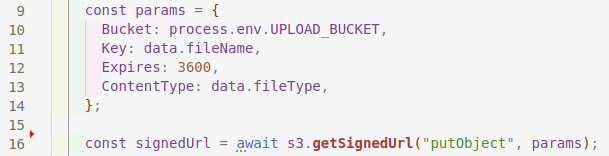
\includegraphics[width=11cm]{immagini/getURL.png} \\
		\caption{\label{fig:getURL} Snippet di codice per ottenere l'URL presigned}
	\end{figure}
	
	Nel codice sopra riportato:
	\begin{itemize}
		\item \textbf{Bucket}: nome del \emph{bucket} su cui effettuare l'operazione;
		\item \textbf{Key}: nome del file che si vuole caricare con il presigned che si ottiene, specificando eventuali prefissi;`
		\item \textbf{ContentType}: tipo del file che si vuole caricare. Nel caso delle immagini caricate da MariBa è \emph{image/jpeg};
		\item \textbf{``putObject''}: tipo di operazione che si vuole effettuare con l'URL generato. In questo caso si 
		tratta di un'operazione PUT.
	\end{itemize}
	Le immagini caricate hanno utilità molto breve: infatti una volta che il back-end ne ha effettuato il \emph{download}, 
	esse non verranno più utilizzate. Di conseguenza, per evitare di lasciare all'interno del \emph{bucket} dell'inutile spazzatura, è stata impostata una \emph{lifecycle rule} in modo tale che tutte le immagini caricate (con prefisso \emph{img/}) vengano eliminate in modo automatico dopo un giorno dal loro caricamento.
	Per informazioni specifiche riguardo alla \emph{lifecycle rule} fare riferimento alla \autoref{subsec:bucketS3}.
	
	\subsubsection{AWS Lambda}
	Di seguito sono descritte le funzioni \emph{Lambda} implementate per il corretto funzionamento della funzionalità di riconoscimento automatico dei giocatori:
	\begin{itemize}
		\item \texttt{getPresignedUpload}: richiede ad \emph{S3} il presigned URL per il caricamento dell'immagine in uno specifico \emph{bucket} e con uno specifico prefisso;
		\item \texttt{callRekognition}: effettua il \emph{download} dell'immagine dal \emph{bucket} S3 in modo che possa essere utilizzata da \texttt{elaborateImage};
		\item \texttt{elaborateImage}: effettua le chiamate effettive a \emph{Rekognition}. In particolare:
			\begin{enumerate}
				\item Individua i volti nella fotografia utilizzando \texttt{rekognition.DetectFaces}, la quale restituisce le relative \emph{bounding box};
				\item Ritaglia i volti individuati utilizzando tali \emph{bounding box};
				\item Per ciascun volto ritagliato chiama \texttt{rekognition.SerachFacesByImage} per cercare eventuali corrispondenze all'interno della \emph{collection} contenente tutti i volti precedentemente salvati;
				\item Se sono state trovate delle somiglianze vengono restituiti i \emph{faceId} corrispondenti in ordine decrescente di probabilità;
				\item Per ciascun volto individuato nell'immagine iniziale restituisce le informazioni sulla relativa bounding box. Inoltre, nel caso fossero state trovate corrispondenze, restituisce anche il \emph{faceId}. In caso contrario restituisce invece i crop dei visi non riconosciuti.
			\end{enumerate}
		\item \texttt{updatePlayer}: aggiorna un giocatore già presente nel database con il nuovo \emph{faceId} nel momento in cui esso viene associato dall'utente;
		\item \texttt{indexFace}: utilizza \texttt{rekognition.IndexFaces} per indicizzare nuove facce all'interno della \emph{collection} di \emph{Rekognition}.
	\end{itemize}
	
	
	
	\subsection{Funzionamento generale}
	Il funzionamento generale del sistema di riconoscimento tramite immagine è schematizzato in \autoref{fig:funzionamento-rek}.
	
	\begin{figure}[H]
		\centering
		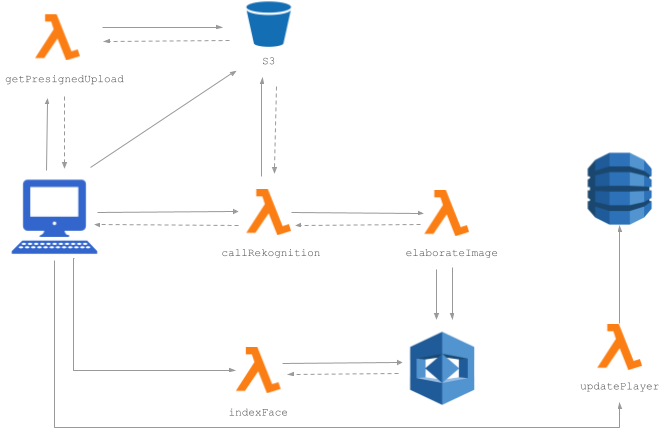
\includegraphics[width=12cm]{immagini/funzionamento.png} \\
		\caption{\label{fig:funzionamento-rek} Grafico del funzionamento del sistema di image recognition}
	\end{figure}

	In particolare avvengono le seguenti operazioni:
	\begin{itemize}
		\item Il front-end utilizza la funzione \texttt{getPresignedUpload} per ottenere l'URL per il caricamento dell'immagine nel \emph{bucket} \emph{S3};
		\item Una volta ottenuto il link, il front-end procede al caricamento;
		\item Chiama la funzione \texttt{callRekognition} e attende i dati delle facce individuate e/o riconosciute;
		\item \texttt{callRekognition} scarica l'immagine dal \emph{bucket} e la passa a \texttt{elaborateImage};
		\item \texttt{elaborateImage} esegue le chiamate effettive a \emph{Rekognition} come descritte nella \autoref{subsec:rekognition};
		\item \texttt{elaborateImage} ritorna il risultato dell'elaborazione opportunamente strutturato a \texttt{callRekognition} che a sua volta lo restituisce al front-end;
		\item Il front-end visualizza i dati ricevuti;
		
		\item Se viene richiesto di registrare un nuovo utente:
		\begin{itemize}
			\item Viene chiamata \texttt{indexFace} per indicizzare il crop del viso non ancora registrato nella \emph{collection} di \emph{Rekognition};
			\item \texttt{indexFace} restituisce il \emph{faceId} del viso indicizzato; 
			\item Viene aggiunto un nuovo record nel database contenente le informazioni del nuovo giocatore, compreso il \emph{faceId} ricevuto;
		\end{itemize}
		
		\item Se viene richiesto di associare un nickname già esistente ad un viso:
		\begin{itemize}
				\item Viene chiamata \texttt{indexFace} per indicizzare il crop del viso non ancora registrato nella \emph{collection} di \emph{Rekognition};
			\item \texttt{indexFace} restituisce il \emph{faceId} del viso indicizzato; 
			\item Viene chiamata \texttt{updatePlayer} per inserire il \emph{faceId} nel record del giocatore da associare. Nel caso in cui vi fosse già un \emph{faceId}, questo viene sostituito.
		\end{itemize}
		
	\end{itemize}
	
		
		
	
	
	\subsection{Design dell'interfaccia}
	Per il design dell'interfaccia, prima della sua effettiva codifica, sono stati realizzati dei \emph{wireframes} utilizzando \emph{Balsamiq}. In questo modo si è potuto definire il flusso di funzionamento a livello di front-end. \\ 

	\noindent Successivamente, la realizzazione dell'interfaccia è avvenuta utilizzando \emph{Angular 12.x} in combinazione con la libreria 
	\emph{Nebular}, specifica per lo sviluppo di interfacce utente. \\
	
	\noindent Nei paragrafi seguenti viene mostrata l'interfaccia realizzata per l'inserimento dei giocatori attraverso l'utilizzo della funzionalità di riconoscimento.
	
		\subsubsection{Inserimento di una nuova partita di calcetto}
		Nella pagina per l'inizializzazione di una nuova partita di calcetto è stato aggiunto un pulsante per attivare la webcam e scattare la foto  contenente i volti dei giocatori (\autoref{fig:calcetto-1}). Lo scatto viene quindi inviato a \emph{Amazon Rekognition} per il riconoscimento facciale. 
		
		\begin{figure}[H]
			\centering
			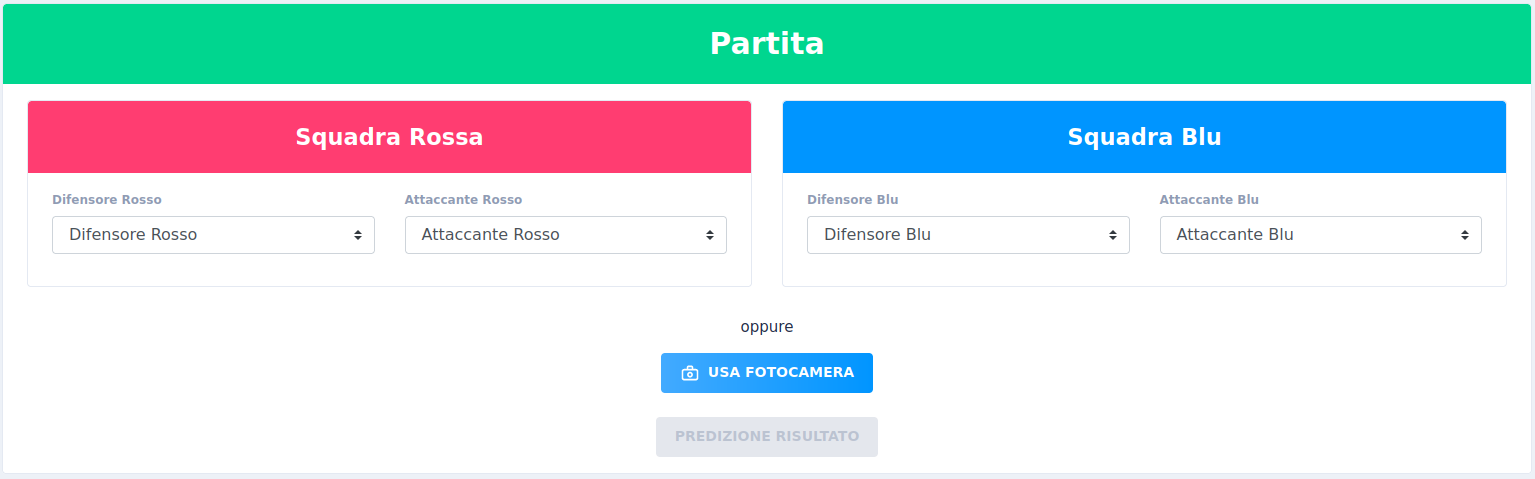
\includegraphics[width=\textwidth]{immagini/calcetto-1.png} \\
			\caption{\label{fig:calcetto-1} Schermata iniziale di calcetto}
		\end{figure}
	
		\noindent Una volta ricevuto il risultato dell'elaborazione, i giocatori vengono visualizzati in card selezionabili per la formazione delle squadre (\autoref{fig:calcetto-2}). I giocatori possono appartenere a tre categorie differenti:
		\begin{itemize}
			\item \textbf{Giocatore riconosciuto}: viene mostrato il nickname corrispondente al volto riconosciuto;
			\item \textbf{Giocatore non riconosciuto ma registrato}: il giocatore è già registrato ma non ha ancora un volto associato. Quando selezionato richiede l'associazione del nickname al viso scegliendo tra i nickname già presenti nel database;  
			\item\textbf{Giocatore non riconosciuto e non registrato}: quando selezionato richiede la registrazione di un nuovo giocatore; 
		\end{itemize}
	
		\noindent Nel caso in cui uno o più giocatori non fossero presenti all'interno della fotografia scattata, è possibile inserirli manualmente. Una volta inserito il nickname desiderato viene mostrata la card corrispondente. \\
		Il numero di giocatori selezionabili per ciascuna squadra è esattamente due. 
		
		\begin{figure}[H]
			\centering
			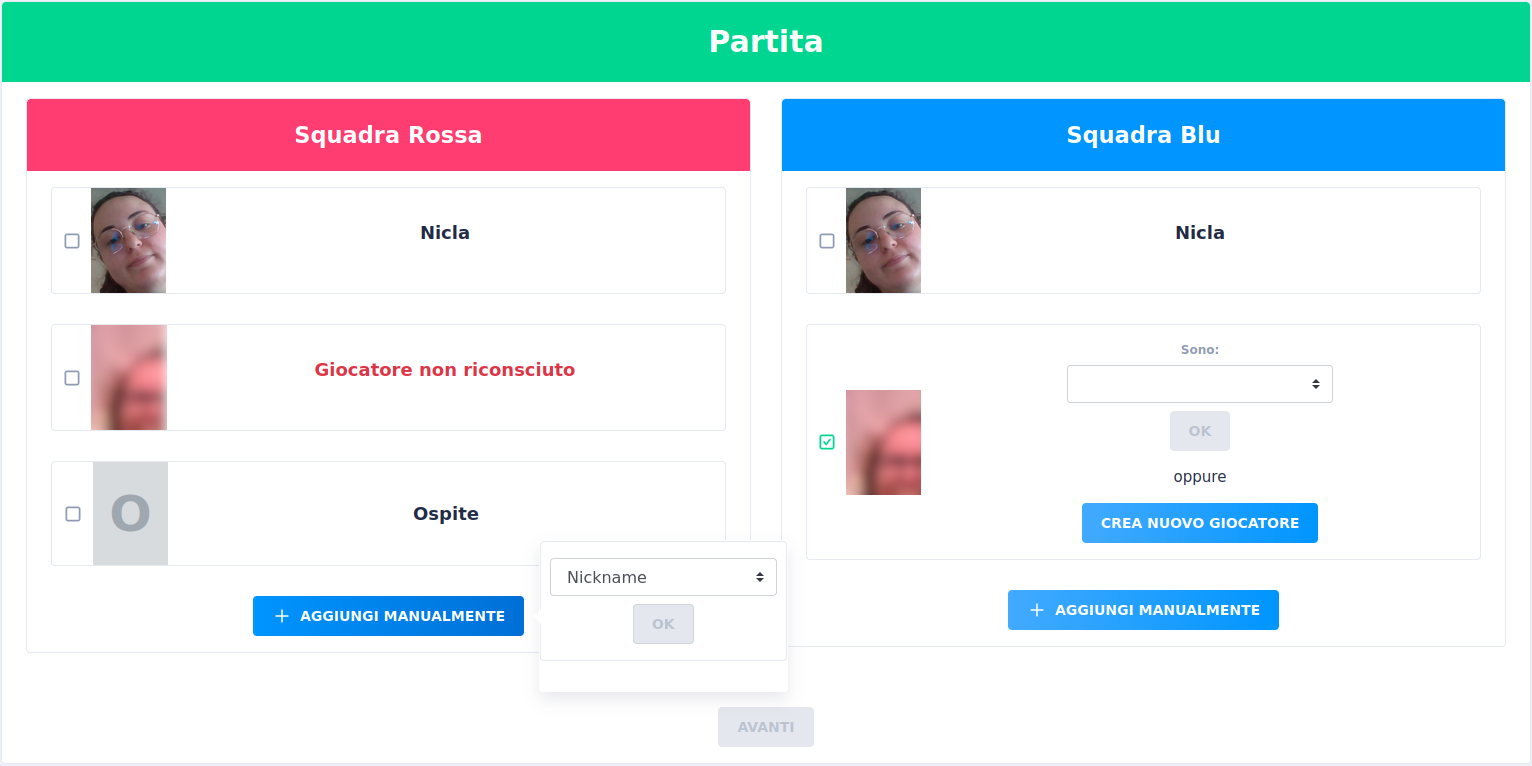
\includegraphics[width=\textwidth]{immagini/calcetto-2.png} \\
			\caption{\label{fig:calcetto-2} Selezione dei giocatori}
		\end{figure}
		
		\noindent Dopo la selezione dei giocatori sarà inoltre possibile scambiare i due nickname all'interno di ciascuna squadra per associare loro il ruolo desiderato e formare le squadre definitive (\autoref{fig:calcetto-3}) .
			
		\begin{figure}[H]
			\centering
			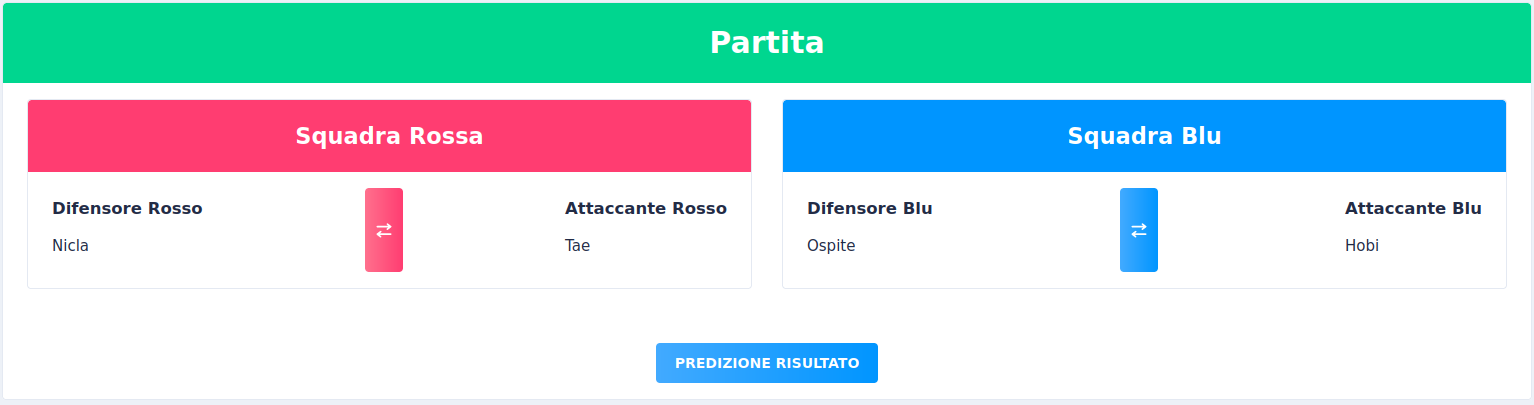
\includegraphics[width=\textwidth]{immagini/calcetto-3.png} \\
			\caption{\label{fig:calcetto-3} Formazione squadre di calcetto}
		\end{figure}
		
		
		\subsubsection{Inserimento di una nuova partita di Mario Kart e Duck Game}
		Il procedimento da seguire per l'inserimento di una partita di Mario Kart o di Duck Game tramite l'utilizzo del riconoscimento facciale dei giocatori è pressoché il medesimo. \\
		La sola differenza tra i due giochi è individuabile nel numero di giocatori selezionabili: 
		\begin{itemize}
			\item per Mario Kart devono essere inseriti esattamente quattro giocatori (\autoref{fig:kart-1});
			\item per Duck Game si possono inserire da un minimo di due ad un massimo di otto giocatori (\autoref{fig:duck-1}).
		\end{itemize}
	
		Ad entrambe le schermate, come per calcetto, è stato quindi aggiunto un pulsante per attivare la webcam e scattare la fotografia da inviare ad \emph{Amazon Rekognition}.
		
		\begin{figure}[H]
			\centering
			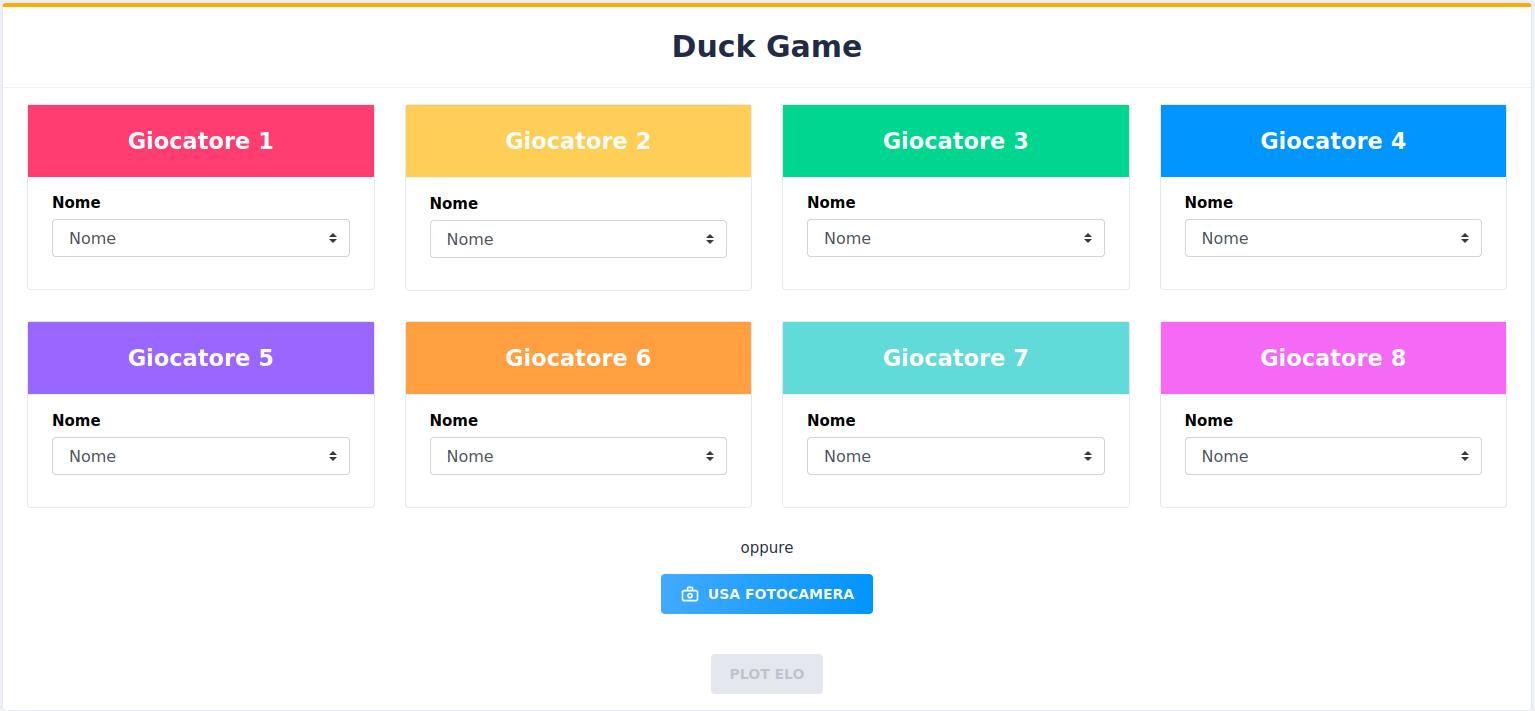
\includegraphics[width=\textwidth]{immagini/duck-1.png} \\
			\caption{\label{fig:duck-1} Schermata iniziale di Duck Game}
		\end{figure}
	
		\begin{figure}[H]
			\centering
			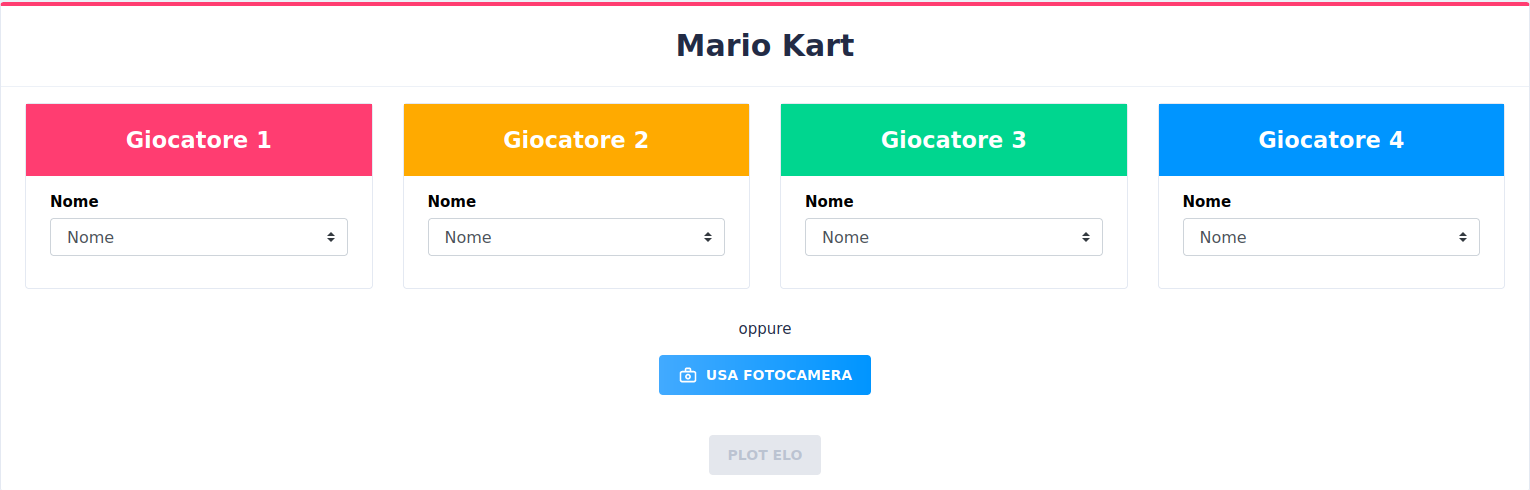
\includegraphics[width=\textwidth]{immagini/kart-1.png} \\
			\caption{\label{fig:kart-1} Schermata iniziale di Mario Kart}
		\end{figure}
		
		\noindent Una volta ricevuto il risultato dell'elaborazione, i giocatori vengono visualizzati in card selezionabili (\autoref{fig:kart-2}). I giocatori possono appartenere a tre categorie differenti:
		\begin{itemize}
			\item \textbf{Giocatore riconosciuto}: viene mostrato il nickname corrispondente al volto riconosciuto;
			\item \textbf{Giocatore non riconosciuto ma registrato}: il giocatore è già registrato ma non ha ancora volto associato. Quando selezionato richiede l'associazione del nickname al viso scegliendo tra i nickname già presenti nel database; 
			\item\textbf{Giocatore non riconosciuto e non registrato}: quando selezionato richiede la registrazione di un nuovo giocatore; 
		\end{itemize} 
	
		\noindent Nel caso in cui uno o più giocatori non fossero presenti all'interno della fotografia scattata, è possibile inserirli manualmente. Una volta inserito il nickname desiderato viene mostrata la card corrispondente.
		
		\begin{figure}[H]
			\centering
			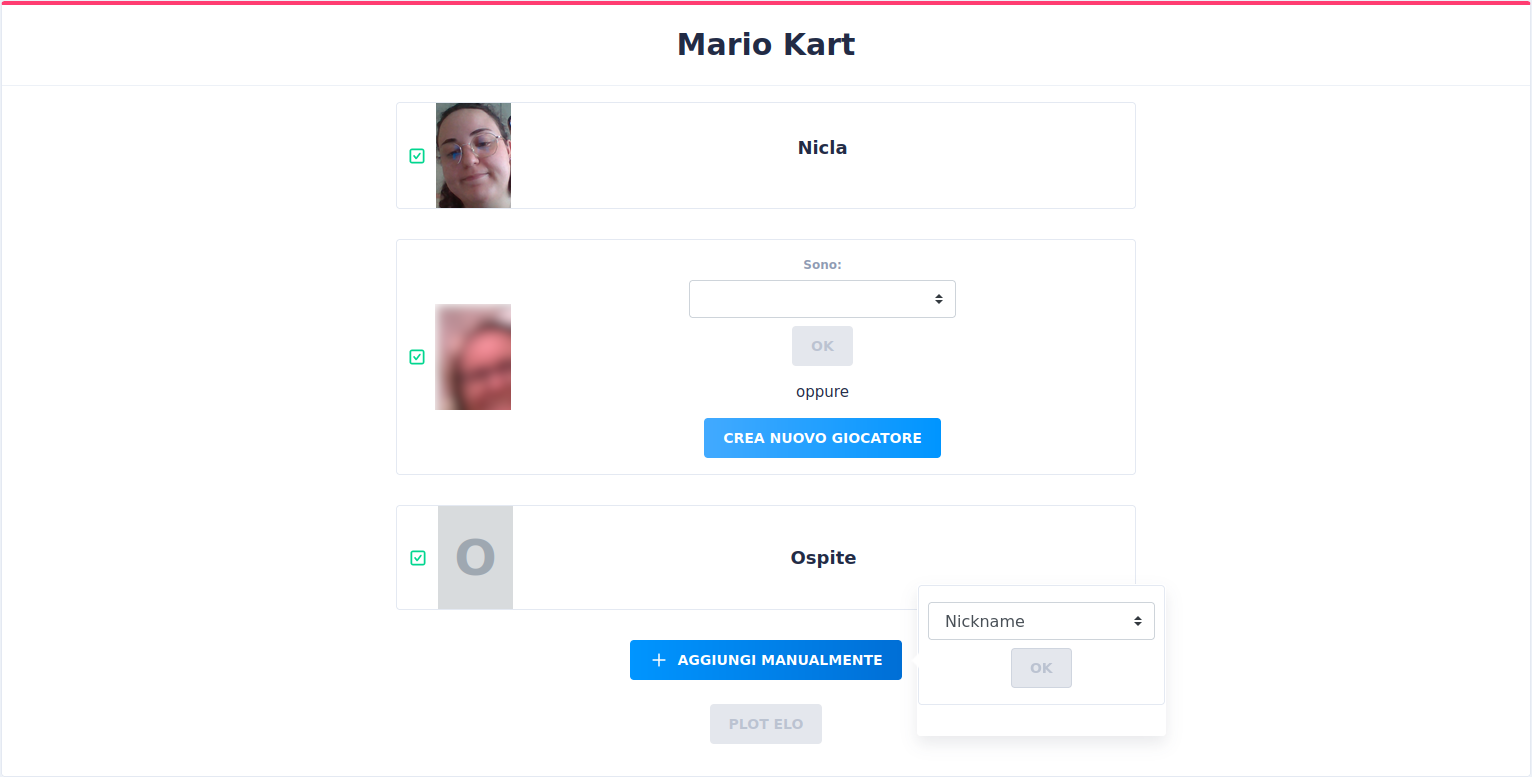
\includegraphics[width=\textwidth]{immagini/kart-2.png} \\
			\caption{\label{fig:kart-2} Selezione dei giocatori di Mario Kart}
		\end{figure}
	
		
				% sviluppo image recognition
% !TEX encoding = UTF-8
% !TEX TS-program = pdflatex
% !TEX root = ../tesi.tex

%**************************************************************
\chapter{Integrazione di Amazon Lex}
\label{cap:lex}
%**************************************************************

In questo capitolo viene approfondito lo sviluppo e l'integrazione del sistema di interazione vocale \\

%**************************************************************

\section{Presentazione del problema}
\section{Progettazione}
	\subsection{Architettura}
	\subsection{Design dell'interfaccia}

				% sviluppo lex

% !TEX encoding = UTF-8
% !TEX TS-program = pdflatex
% !TEX root = ../tesi.tex

%**************************************************************
\chapter{Conclusioni}
\label{cap:conclusioni}
%**************************************************************

%**************************************************************
\section{Consuntivo finale}

\begin{center}
	
	\renewcommand{\arraystretch}{1.5}
	
	\centering
	\begin{longtable}{| C{2.5cm} | C{2cm} | L{7.2cm} |}
		
		\hline
		
		\rowcolor{lighter-bugBlue}
		\textbf{Durata in ore} & \textbf{Settimana} & \textbf{Descrizione} \\
		
		\hline
		
		40 & 1 &
		\begin{itemize}[leftmargin=*]
			\item Studio delle tecnologie necessarie.
		\end{itemize} \\
		
		\hline
		
		100 & 2, 3, 4 &
		\begin{itemize}[leftmargin=*]
			\item Progettazione e sviluppo di un micro-servizio per attività di \emph{face detection} per 
			la creazione di squadre di gioco;
			\item Integrazione con la piattaforma esistente. 
		\end{itemize}  \\
		
		\hline
		
		40 & 4, 5 &
		\begin{itemize}[leftmargin=*]
			\item Progettazione e sviluppo di una sezione del sito per l'inserimento dei risultati di un nuovo gioco;
			\item Integrazione con la piattaforma esistente. 
		\end{itemize}  \\
		
		\hline
		
		100 & 5, 6, 7 &
		\begin{itemize}[leftmargin=*]
			\item Progettazione e sviluppo di un micro-servizio per il controllo vocale;
			\item Integrazione con la piattaforma esistente. 
		\end{itemize}  \\
		
		\hline
		
		40 & 8 &
		\begin{itemize}[leftmargin=*]
			\item Stesura della documentazione di progetto delle attività di sviluppo condotte nelle settimane precedenti.
		\end{itemize} \\
		
		\hline
		
		\rowcolor{lighter-bugBlue}
		\multicolumn{2}{| c | }{\textbf{Totale ore: }} & 	\multicolumn{1}{  c | }{\textbf{320}}\\
		
		\hline
		
		
		\caption{Pianificazione delle attività}
	\end{longtable}
	
	
\end{center}

%**************************************************************
\section{Raggiungimento degli obiettivi}

%**************************************************************
\section{Conoscenze acquisite}

%**************************************************************
\section{Valutazione personale}
             % Conclusioni


%**************************************************************
% Materiale finale
%**************************************************************
\backmatter
\printglossaries
% !TEX encoding = UTF-8
% !TEX TS-program = pdflatex
% !TEX root = ../tesi.tex

%**************************************************************
% Bibliografia
%**************************************************************

\cleardoublepage
\chapter{Bibliografia}

\nocite{*}

% Stampa i siti web consultati
\printbibliography[heading=subbibliography,title={Siti web consultati},type=online]


\end{document}
